\documentclass[conference,letterpaper,10pt]{./../../IEEE/IEEEtran}

\usepackage{graphicx}
\usepackage{amsmath}
\usepackage{amsfonts}
\usepackage{algorithm}
\usepackage{algorithm,acronym}
\usepackage{subeqnarray,cite,mathtools,url,multirow}

\graphicspath{{./../Figures/}}
\DeclareGraphicsExtensions{.pdf}

\acrodef{MSE}{mean squared error}
\acrodef{IBC}{interference broadcast channel}
\acrodef{MC}{multi-cell}
\acrodef{BS}{base station}
\acrodef{MIMO}{multiple-input multiple-output}
\acrodef{SISO}{single-input single-output}
\acrodef{MU}{multiple users}
\acrodef{OFDM}{orthogonal frequency division multiplexing}
\acrodef{WSRM}{weighted sum rate maximization}
\acrodef{QoS}{quality of service}
\acrodef{SCA}{successive convex approximation}
\acrodef{SNR}{signal-to-noise ratio}
\acrodef{MMSE}{minimum \acl{MSE}}
\acrodef{SIR}{signal-to-interference ratio}
\acrodef{SINR}{signal-to-interference-plus-noise ratio}
\acrodef{Q-WSRM}{queue \acl{WSRM}}
\acrodef{QM}{queue minimizing}
\acrodef{SRA}{spatial resource allocation}
\acrodef{JSFRA}{joint space-frequency resource allocation}
\acrodef{WMMSE}{weighted \acl{MMSE}}
\acrodef{KKT}{Karush-Kuhn-Tucker}
\acrodef{GP}{geometric programming}
\acrodef{SOC}{second-order cone}
%\acrodef{BCDM}{block coordinate descent method}
\acrodef{ADMM}{alternating directions method of multipliers}
\acrodef{PD}{primal decomposition}
\acrodef{DD}{dual decomposition}
\acrodef{FFR}{fractional frequency reuse}
\acrodef{DC}{difference of convex}
\acrodef{Q-WSRME}{\ac{Q-WSRM} extended}
\acrodef{TDD}{time division duplexing}
\acrodef{CSI}{channel state information}
\acrodef{AO}{alternating optimization}
\acrodef{OTA}{over-the-air}
\acrodef{PL}{path loss}
\acrodef{TDM}{time division multiplexing}
\acrodef{UC}{uncoordinated}
\acrodef{SoC}{system-on-chip}
\acrodef{WMMSE}{weighted minimum mean squared error}
\acrodef{AMBA}{Advanced Microcontroller Bus Architecture}
\acrodef{AXI}{Advanced Extensible Interface}
\acrodef{FPGA}{Field-programmable gate array}
\acrodef{MSMCSRAM}{multi-core shared memory}
\acrodef{IPC}{inter-processor communications}
\acrodef{CIC}{chip-level interrupt controller}
\acrodef{MCSDK}{multi-core software development kit}
\acrodef{AMP}{Asymmetric Multi-Processing}
\newcommand{\mbf}[1]{\mathbf{#1}}
\newcommand{\me}[1]{\( #1 \)}
\newcommand{\mc}[1]{\mathcal{#1}}
\newcommand{\fall}{\forall}
\newcommand{\set}[1]{\left \lbrace #1 \right \rbrace }
\newcommand{\mvec}[2]{\mathbf{#1}_{#2}}
\newcommand{\ith}[1]{{#1}^\mathrm{th}}
\newcommand{\pr}[1]{{#1}^\prime}
\newcommand{\mbfa}[1]{{\boldsymbol{#1}}}
\newcommand{\herm}{\mathrm{H}}
\newcommand{\sset}[1]{\left [ #1 \right ]}
\newcommand{\rfrac}[2]{{}^{#1}/{}_{#2}}
\newcommand{\eqspace}{\IEEEeqnarraynumspace}
\newcommand{\enoise}{\widetilde{N}_0}
\newcommand{\eqsub}{\IEEEyessubnumber}
\newcommand{\review}[1]{{\textcolor[rgb]{0 0 0.6}{#1}}}
\newcommand{\trace}{\mathrm{tr}}
\newcommand{\tran}{\mathrm{T}}
\newcommand{\R}[1]{\label{#1}\linelabel{#1}}
\newcommand{\lr}[1]{page~\pageref{#1}, line~\lineref{#1}}
\newcommand{\eqn}[1]{\(#1\)}
\newcommand{\mx}{\mbf{m}}
\newcommand{\my}{\mbf{w}}
\newcommand{\mz}{\mbfa{\gamma}}
\newcommand{\mxb}{{{\mbf{m}}}}
\newcommand{\myb}{{{\mbf{w}}}}
\newcommand{\iterate}[2]{{#1}^{(#2)}}
\newcommand{\iter}[3]{{#1}_{#2}^{(#3)}}
\newcommand{\ma}{\mbf{x}}

\begin{document}

\title{Implementation of MU-MIMO Schedulers on SoC}
%\vspace{-22ex}

\author{\begin{tabular}{cc}
\multicolumn{2}{c}{Ganesh Venkatraman, Janne Janhunen, and Markku Juntti}\\
Centre for Wireless Communications (CWC), & Department of Communication Engineering (DCE), \\
\multicolumn{2}{c}{FI - 90014, University of Oulu, Finland}\\
\end{tabular}}

\maketitle

\begin{abstract}
To avail the benefits of a multi-antenna system, \ac{MU} \ac{MIMO} systems multiplex different user data streams spatially over time-frequency resources. However, serving dozens of users with spatial multiplexing increases the scheduler complexity significantly. In this work, we demonstrate the computational requirements of different state-of-the-art MU-MIMO scheduling algorithms and evaluate the number of users that can be supported in real-time. To provide a fair comparison, we initially analyze the achievable sum rate of various scheduling algorithms using MATLAB for different MIMO configurations. We also propose a modification to the existing scheduling algorithm to improve the sum rate. We then implement the scheduling algorithms on Xilinx ZYNQ-ZC702 \ac{SoC} to illustrate the advantages.
\end{abstract}

\acresetall
\section{Introduction}
The current wireless standards are moving towards the packet switched networks to improve the system performance and flexibility as compared to the circuit switched networks. The radio access technologies aim at achieving higher throughput and better system performance but still targeting to low energy budget. The use of multi-antenna transmission is \textit{de-facto} in all upcoming wireless access standards, favoring the spatial multiplexing of user data by applying transmit precoders for \ac{MU} \ac{MIMO} transmission. In order to achieve the best possible benefit of the multi-user \ac{MIMO} transmission, the multiplexed users should have channel vectors as linearly independent as possible. 
By selecting users with the uncorrelated channel vectors, efficient linear precoders can be designed to decouple the user data streams and to avail the benefits of MU-MIMO technique. The selection of users with such a constraint is carried out by the schedulers to utilize the wireless system resources efficiently.

The scheduling algorithms based on sum rate maximization objective for MU-MIMO were discussed thoroughly in the literature. The search based on successive projections (SP) scheme for single-antenna receiver was presented in \cite{sus2006zfbf} and its extension to the multi-antenna receivers was provided in \cite{Tolli-etal-2005}. In \cite{Tolli-etal-2005}, the users were selected iteratively by choosing the channel vector with the maximum gain on to the orthogonal subspace. The orthogonal subspace was obtained by evaluating the null space of the stacked channel vectors of the already chosen users from the earlier iterations. Similar algorithms addressing a lower computational complexity were proposed in \cite{shen2006low} and \cite{youtuan2007improved}. User selection based on the volume maximization metric was discussed in \cite{jin2010novel}. The performance of the volume based selection is identical to the SP or block diagonalization (BD) scheme, since both schemes use the Gram-Schmidt (GS) procedure.

We evaluate the performance of the scheduling algorithms by the achievable sum rate. The iterative precoder design based on \ac{WMMSE} reformulation for the \ac{WSRM} objective provides an efficient transmit precoder design to achieve improved performance \cite{wmmse_shi}. However, the computational complexity involved in the \ac{WMMSE} design is large in comparison to the elementary zero-forcing (ZF) based precoder design proposed in \cite{spencer2004zero}. Even though the ZF based precoder design is inferior to the \ac{WMMSE} approach, it provides a closed form expression to evaluate the precoder design followed by a bisection search to identify the power for each data stream. The choice of precoder design also plays a major role in the achievable sum rate. In the current work, we rely on the ZF based precoder design as compared to the iterative WMMSE approach.

In this paper, we study the computational complexity of different state-of-the-art MU-MIMO scheduling algorithms and evaluate the number of users that can be served in the system. To enable a fair comparison, we first analyze the achievable sum rate performance of the different algorithms and then we discuss the implementation of the scheduling schemes on Xilinx ZYNQ 7000 ZC702 \ac{SoC} to show how the current systems can take advantage of MU-MIMO techniques. This work is a continuation to our previous implementation studies \cite{Janhunen-etal-11, Hanninen-etal-2014, Shahabuddin-etal-2014} aiming at finding low-power but high performance solutions for the advanced long term evolution (LTE-A) transceivers. Current work excludes precoding implementation, but we considered a two-step scheduling-precoding design approach, where the scheduler identifies a subset of users in the first step and then the precoders are designed for the chosen subset in the second step.

The paper is organized as follows. A single-cell downlink system model is described in Section \ref{sec:system_model} followed by a brief discussion on the scheduler algorithms in Section \ref{sec:sched_discussions}. Section \ref{sec:perf_scheduling} presents the performance comparison between selected scheduler schemes using link level simulations. In Section \ref{sec:implementation}, implementation results of different scheduling algorithms are presented. Section \ref{sec:conclusion} summarizes the conclusions and future work.

\section{System Model}
\label{sec:system_model}
We consider a single-cell downlink MU-MIMO transmission with \eqn{N_T} transmit antennas and \eqn{N_K} users with \eqn{N_R} antenna each. Let \eqn{\mvec{H}{k} \in \mathbb{C}^{N_R \times N_T}} be the channel matrix seen by user \me{k}. Let \me{\kappa = \min(N_R,N_T)} be the rank of the channel matrix \me{\mvec{H}{k}}. In order to perform scheduling over multiple spatial streams, the channel matrix \eqn{\mvec{H}{k}} is decomposed into \me{N_R} virtual single antenna receiver channels using singular value decomposition (SVD) as \eqn{\mvec{H}{k} = \mvec{U}{k} \mvec{D}{k} \mvec{V}{k}^\herm}, where \eqn{\mvec{U}{k} \mvec{U}{k}^\herm = \mbf{I}_{N_R}} and \eqn{\mvec{V}{k}\mvec{V}{k}^\herm = \mbf{I}_{N_T}} are unitary matrices and \eqn{\mvec{D}{k}} is a diagonal matrix. 
The virtual user index for the \me{\ith{i}} column vector of \me{\mvec{U}{k} \in \mathbb{C}^{N_R \times N_R}} of the \me{\ith{k}} user is denoted by \me{\hat{k} = k \kappa + i} and the equivalent single antenna receiver channel is \eqn{\mvec{h}{\hat{k}} = \mvec{U}{k}(i)^\herm \mvec{H}{k}}. The total number of virtual single antenna users in the system is given by \eqn{K = \kappa N_K}. Let \eqn{\mc{U}} be the set of indices of the users present in the system and let \eqn{\mc{A} \subset \mc{U}} be the set of active users chosen by the scheduling algorithm for a transmission instant. For brevity, the virtual users are referred as users in the forthcoming discussion. Now, the equalized received symbol \eqn{\hat{d}_k} of user \me{k \in \mc{A}} is given by
\begin{equation}
\hat{d}_k = \mvec{h}{k} \mvec{m}{k} d_k + \sum_{i \in \mc{A} \backslash \{k\}} \mvec{h}{k} \mvec{m}{i} d_i + {n}_{k},
\end{equation}
where \eqn{{n}_{k} \in \mathbb{C}} is the equivalent zero mean complex Gaussian noise with variance \eqn{\mc{N}(0,N_0)} and \me{\mvec{m}{k} \in \mathbb{C}^{N_T \times 1}} is the transmit precoder corresponding to user \me{k}. The data symbol \me{d_k} is assumed to be uncorrelated with \me{\mathrm{E}[|d_k|^2] = 1}.

\section{Scheduling Algorithms}
\label{sec:sched_discussions}
The selection of a subset of users \eqn{\mc{A}} from \eqn{\mc{U}} is a combinatorial problem in general. Therefore it requires the complexity of \eqn{O(K^{N_T})}. Fig. \ref{kuva:scheduler_block_diag} shows the outline of scheduling algorithms discussed in this section. Due to the simplicity of the greedy/norm based search, we omit the discussion on the greedy scheduling algorithm.
\begin{figure}
	\centering
	%trim=0in 0.25in 0in 0.5in,width=\columnwidth, angle=0	
	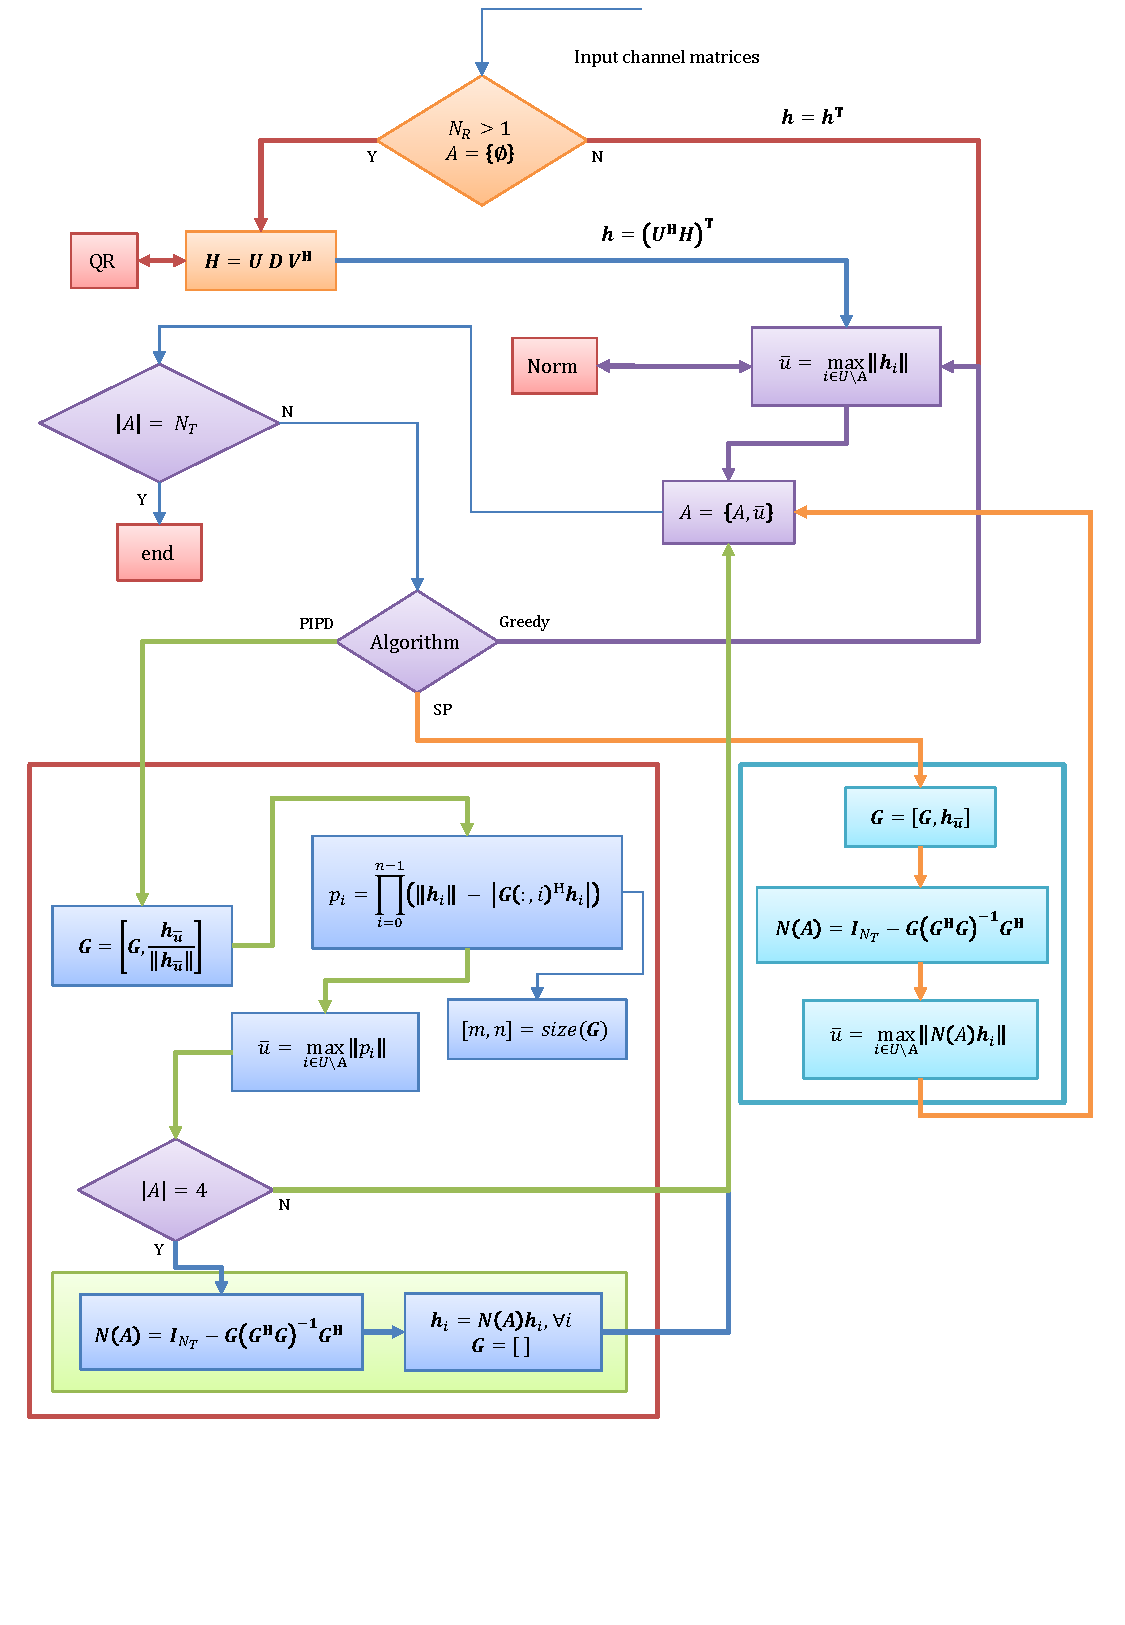
\includegraphics[trim=0in 1.5in 0in 0.0in,width=\columnwidth, angle=0]{Algorithm_Model}
	\caption{Block diagram of the scheduler algorithms: greedy, product of independent projections and successive projections.}
	\label{kuva:scheduler_block_diag}
	 \vspace{-0.1in}
\end{figure}

\subsection{Successive Projections}
In the iterative SP selection algorithm, the compatibility of the user channel vectors are evaluated by projecting the channel vector onto the null space formed by stacking the existing channel vectors of the chosen users from the earlier iteration \cite{sus2006zfbf,antti_user_selection}. Initially, a user with higher channel gain from the set \me{\mc{U}} is selected for the transmission set \me{\mc{A}}. Then, the remaining users are selected from \eqn{\mathcal{U} \backslash \mathcal{A}} by projecting the equivalent channel vectors \me{\mvec{h}{\hat{k}} =\mvec{U}{k}(i)^\herm \mvec{H}{k}} on to the null space of the channel vectors of chosen users in \eqn{\mathcal{A}} as
\begin{subeqnarray}
\mbf{F} &=& \left [ \mvec{h}{\mathcal{A}(1)}^\tran,\dotsc,\mvec{h}{\mathcal{A}(|\mathcal{A}|)}^\tran \right ] \slabel{eqn-1.0} \\
\mbf{N}(\mathcal{A}) &=& \mbf{I}_{N_T} - \mbf{F} \left (\mbf{F}^\herm \mbf{F} \right )^{-1} \mbf{F}^\herm \slabel{eqn-1.1}
\end{subeqnarray}
where \textbf{N} denotes the null space matrix and $\mbf{I}_{N_T}$ is the identity matrix of size $N_T$. The metric used for the user selection is given by
\begin{subeqnarray}
m_i &=& \| \mbf{N}(\mathcal{A}) \, \mvec{h}{i}^\tran \|, \; \forall \, i \, \in \mathcal{U} \backslash \mathcal{A} \label{eqn-1.2}\\
\bar{u} &=& \underset{i}{\arg \max} \; m_i, \quad \mathcal{A} = \mathcal{A} \cup \set{\bar{u}}.
\end{subeqnarray}
The above metric is evaluated for all users at each iteration to identify a user until the condition $|\mc{A}| = N_T$ is satisfied. Even though selecting \me{N_T} users is not optimal in the lower \ac{SNR} regime, the precoders can be recalculated by retaining the channel vectors with non-zero power.

\subsection{Product of Independent Projections (PIPD)}
The PIPD algorithm requires minimal computational complexity compared to the SP scheduling scheme as discussed in \cite{venkatraman2014low}. The complexity involved in selecting the first user remains the same, since the user with the highest channel norm is considered for the set \eqn{\mc{A}} in both schemes. The complexity involved in selecting the remaining users for set \me{\mc{A}} is significantly reduced in the PIPD scheduling scheme by virtue of using the product of independent vector projection displacements metric. A detailed description of the algorithm can be found in \cite{venkatraman2014low}. However, for a system configuration of \me{N_T = 8} antennas, the performance of the PIPD scheme is significantly inferior to that of the SP scheduling algorithm. To overcome this problem, we modified the PIPD algorithm as highlighted in Fig. \ref{kuva:scheduler_block_diag} by projecting user channel vectors on to the null space of existing users channel only when \me{|\mc{A}| = 4}. 

Fig. \ref{kuva:scheduler_block_diag} illustrates the operations involved in the metric calculations for greedy, SP and PIPD scheduling schemes. The blocks mentioned separately for the PIPD and the SP schemes are executed based on the selected algorithm. Greedy algorithm requires only the norm calculation of the virtual channel vectors with which the sorting operation can be used to find the leading $N_T$ users for set $\mathcal{A}$. In case of the SP selection scheme, the users are identified by projecting the corresponding channel vectors onto the null space of the existing users, channel vectors and selecting the one with the maximum projection gain. In order to evaluate the null space, a matrix inversion is needed, which requires significant amount of complexity as compared to the vector multiplications involved in the PIPD algorithm in Fig. \ref{kuva:scheduler_block_diag}.

\section{Performance of MU-MIMO Scheduling}
\label{sec:perf_scheduling}
\subsection{Scheduling Resolution}
The scheduling is performed over scheduling blocks (SBs) and the resolution of a SB significantly affects the performance of the overall throughput. For instance, if the SB resolution is equal to physical resource block (PRB), the scheduling complexity increases linearly with the number of SBs and the throughput performance depends on the number of users in the system. Thus, if the number of users is large, the performance will improve by utilizing the multi-user diversity with the help of a proper scheduling scheme. However, if the users are few in number, the performance degradation is quite significant due to the smaller coding length and lack of channel variations over the smaller SB to extract the channel diversity in the form of coding gain. In case of larger SB size with grouped PRBs, the scheduling complexity will be reduced significantly but the network throughput will also reduce noticeably, unless the channel fading over frequency domain is flat or nearly flat. In this case, the users with the transmission in such scheduling will attain higher throughput due to the longer coding length which needs to be quantified by the system level study.
\begin{figure}
\centering
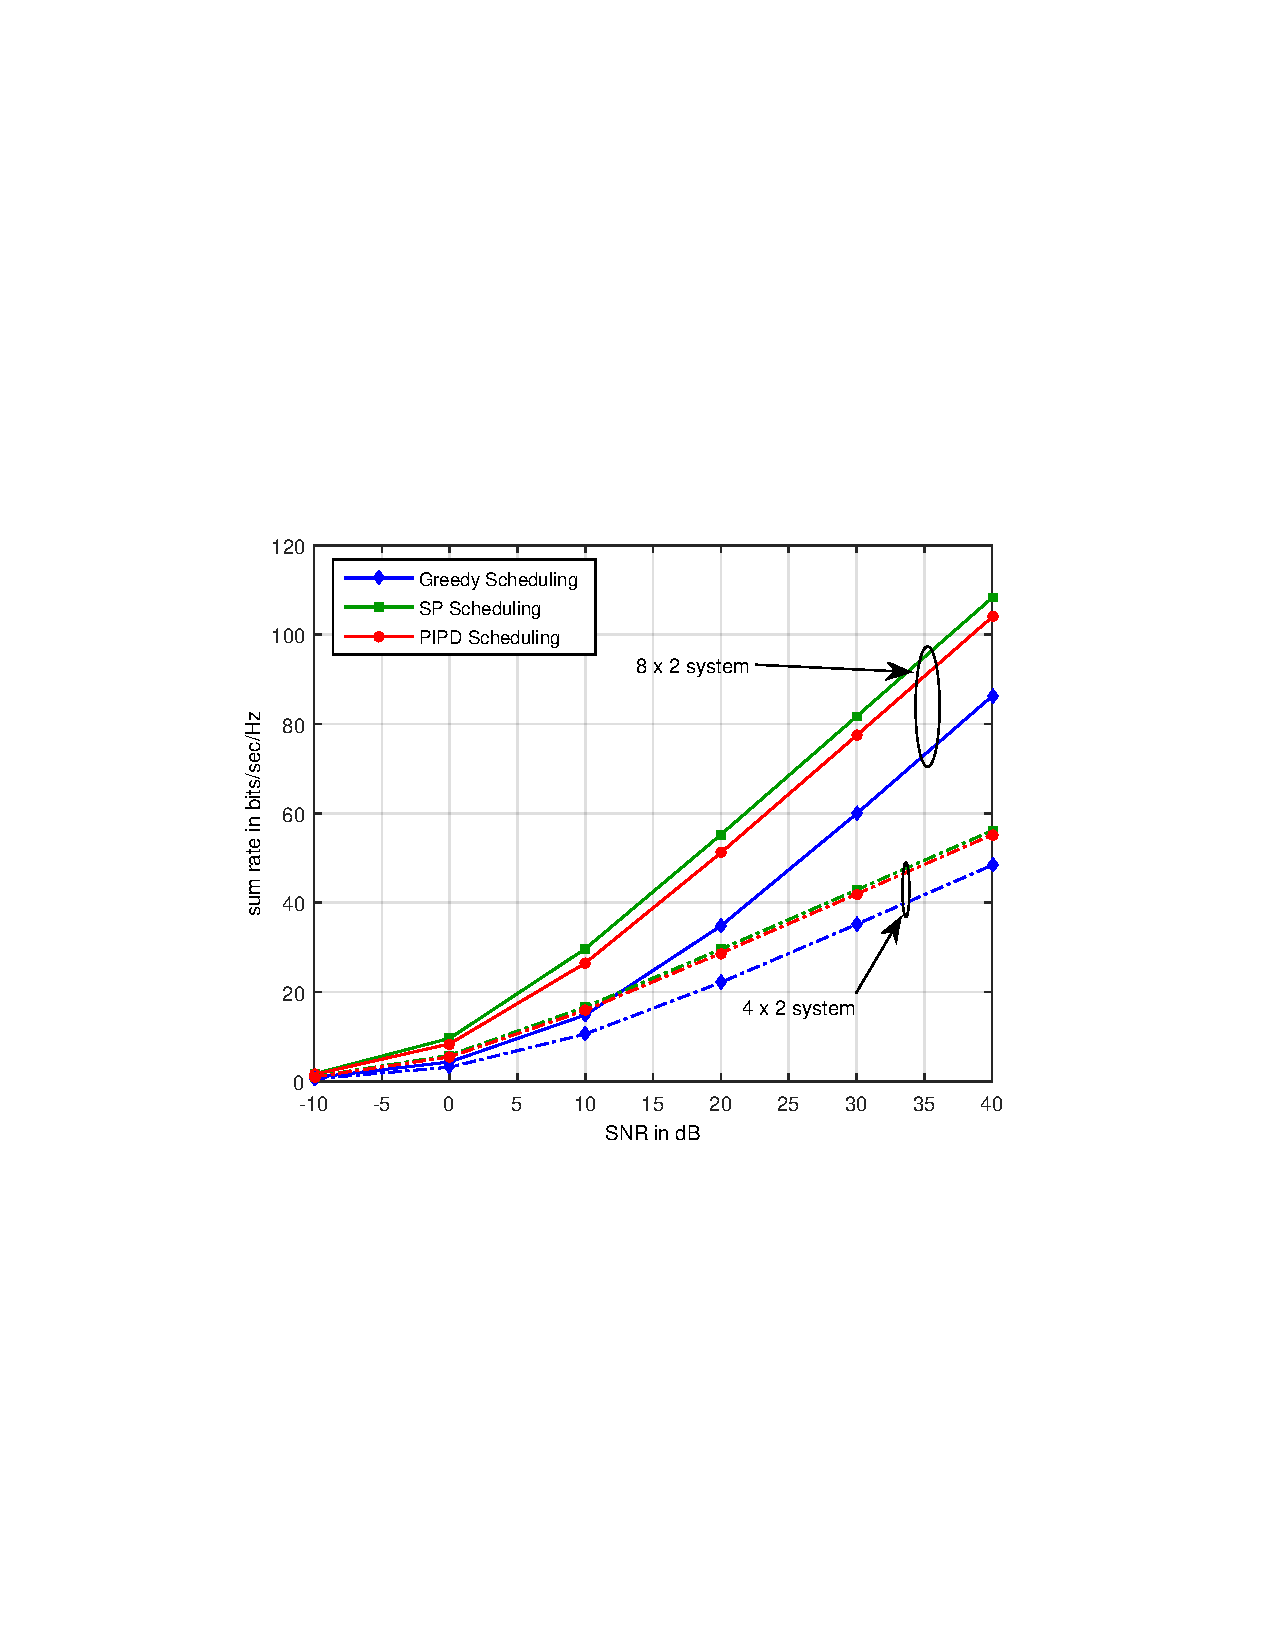
\includegraphics[trim=1.5in 3.5in 1.5in 3.5in,width=\columnwidth]{sra_50_users}
%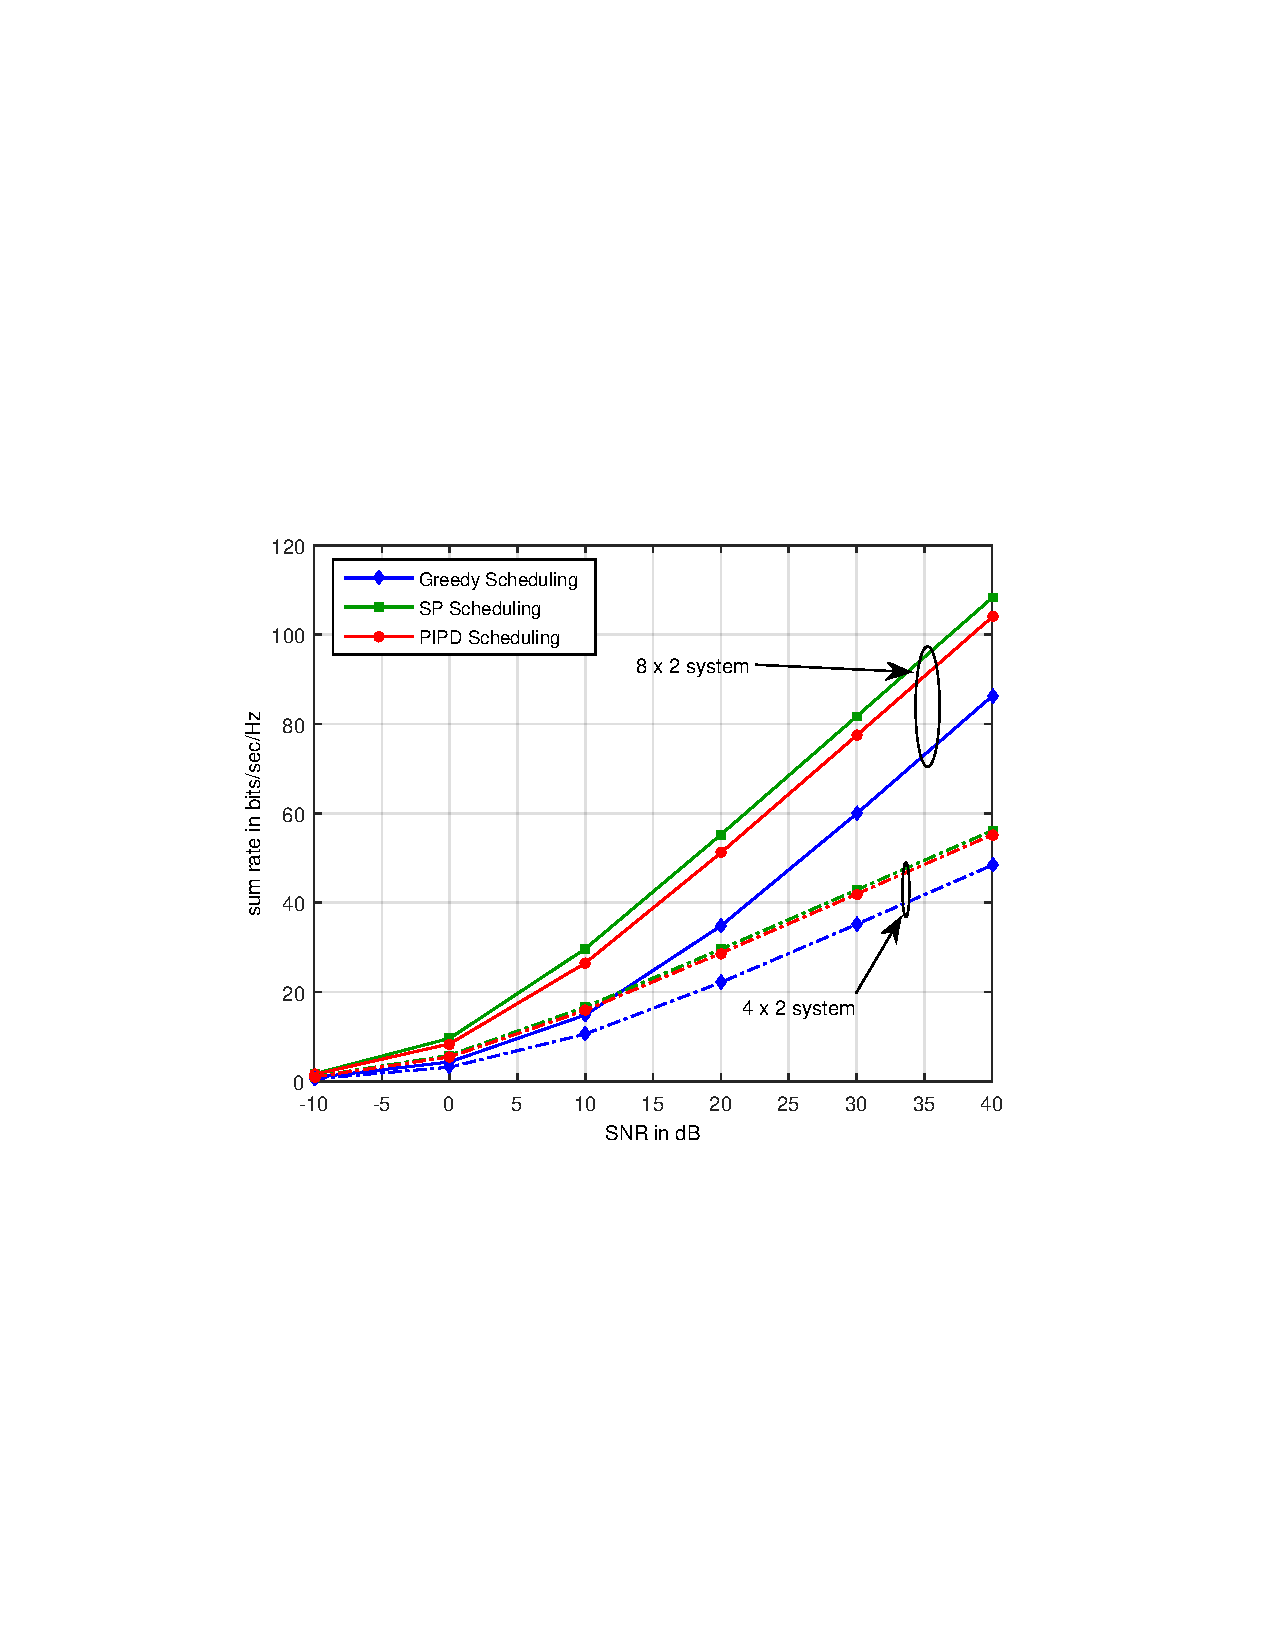
\includegraphics[width=\columnwidth]{sra_50_users}
\caption{Comparison of scheduler algorithms for $N_K = 50$ users.}
\label{kuva:performance_plot}
 \vspace{-0.15in}
\end{figure}

\subsection{Scheduling Performance}
Fig. \ref{kuva:performance_plot} compares the sum rate performance of three different scheduling schemes with $\textrm{N}_T = 4,8$ and $N_K = 50$ users. The sum rate of the PIPD scheme performs remarkably close to the SP scheme. Fig. \ref{kuva:performance_plot} also shows a larger gap (approximately 10 bit/sec/Hz) between Norm/Greedy scheme which selects users based on the channel norm only and PIPD scheduling scheme. Note that the performance of the scheduling algorithms improves marginally by adding additional receive antennas, due to the channel hardening by the multi-user diversity. Increasing \me{N_T} antennas in the system, improves the achievable sum rate of the system by multiplexing more number of users over the spatial dimension, which is evident from Fig. \ref{kuva:performance_plot}.
\begin{figure}
	\centering
	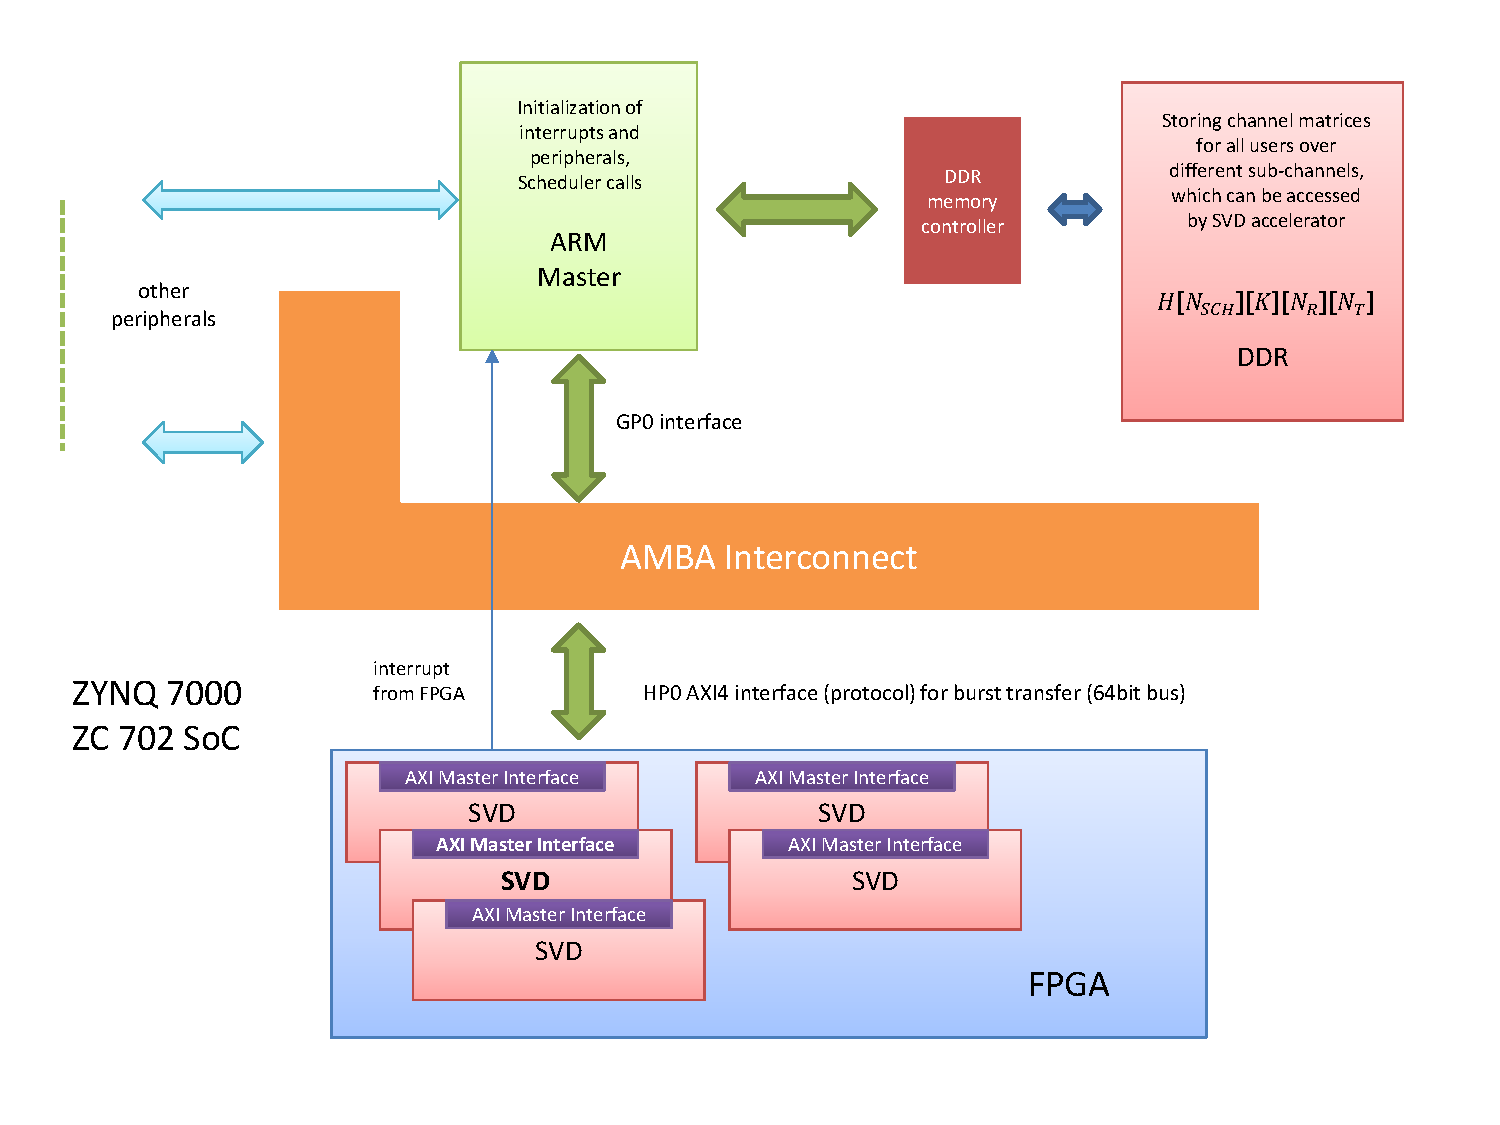
\includegraphics[trim=.75in .75in .75in .75in,width=\columnwidth]{blk_diag}
	\caption{Software and hardware partitioning on ZYNQ 7000.}
	\label{kuva:block_diag}
\end{figure}

\section{Implementation Results}
\label{sec:implementation}
\subsection{ZYNQ ZC702 SoC Evaluation Platform}
The MU-MIMO scheduler algorithms are implemented on the ZYNQ ZC702 SoC, which has dual core ARM processing subsystem (PS) and programming logic (PL) that are interconnected by \ac{AMBA} architecture bus \cite{zynq}. In this study, we limit our scheduler implementation to a single ARM PS only and utilize the maximum available resources of the PL in the board. The ARM PS is operating at $667$ MHz and the PL operates at $100$ MHz. The interconnect between the ARM PS and the PL is via \ac{AXI} \ac{AMBA} interface bus. There are several high performance (HP) buses between the PS and the PL subsystems to reduce the transfer latency. We used HP$0$ interface to interconnect the accelerators implemented on PL to access the DDR memory, where the intended data are stored for the common access.

\subsection{Algorithm Partitioning between ARM PS and PL subsystem}
In this work, we consider performing SVD processing on PL subsystem and scheduling algorithms implementation on ARM PS for the following reasons. Primarily, scheduling algorithms involve sequential processing. Even though metric calculations can be performed in parallel, the maximum metric needs to be obtained over all parallel processing chains to select a candidate user. Note that the NEON vector floating point (VFP) co-processor supports up to \eqn{8} lanes that can perform \eqn{8} computations and searches in parallel, and therefore it would be beneficial to consider PS implementation for less complex parallel implementations. Moreover, scheduling is required for every sub-frame, since it depends on the current number of backlogged packets. On the contrary, SVD processing is required only when the channel matrices change, \textit{i.e.}, once in every \eqn{T_k} sub-frames, where \eqn{T_k} denotes the periodicity of uplink sounding pilots to measure channel that is based on Doppler frequency. Upon considering the above reasons, it would be beneficial to implement scheduling algorithms on ARM PS and SVD processing on PL subsystem.

\subsection{SVD Implementation on PL}
The SVD is performed by repeated QR factorization to obtain left and right singular vectors of the channel matrices. The complex QR decomposition is performed using the Householder transformations \cite{aft}. Since the SVD incurs significant complexity and computational time, it is beneficial to implement on the PL. We use Vivado high-level synthesis (HLS) tool to implement SVD using C. To minimize the resource utilization and to optimize the speed through pipelined processing, respective directives are used in the HLS model.

The choice of fixed point implementation is considered over floating point design for the following reasons. At first, to implement a floating point multiply and accumulate (MAC) operation, LogiCORE IP requires three \textit{DSP48} units, whereas fixed point implementation needs only one DSP48 unit by considering INT16 data format. Secondly, the precision required for real and imaginary part of channel entries can be limited to \eqn{16} bits, since the output resolution of analog-to-digital converter (ADC) is typically in the order of \eqn{14} bits. Therefore, considering the above two facts, we performed SVD implementation using fixed point representation. The fixed point version uses \eqn{18} bit signed representation for real and imaginary components with \eqn{15} bit fractional part and $2$ bit for the integer. To improve the dynamic range of the accelerator, intermediate variables are stored in \eqn{25} bit extended format with \eqn{9} bit for the integer part and one bit for the sign without altering the fractional part share. It would be ideal to store intermediate values in the extended form, since one \textit{DSP48} can perform \eqn{25 \times 18} multiplication without compromising on the resource utilization and the dynamic range involved in the MAC operations \cite{zynq}. 

The SVD accelerator is designed to perform multiple SVD operations with a single trigger from ARM PS. AXI-\textit{Lite} interface is used to provide control information, including matrix size, number of matrices, and streams required, to PL accelerator from ARM PS. Once the control information is processed, matrices are fetched from DDR memory to local BRAM for SVD processing by the PL subsystem. To decompose the channel matrices of all users, we implement five SVD accelerators in parallel to improve the overall throughput of the PL implementation. The restriction on total count of accelerators is due to the resource limitations imposed by the ZC702 board as outlined in Table \ref{tbl-utilization}. Each SVD accelerator is connected as AXI-\textit{Master} to DDR memory via a $64$ bit HP$0$ bus interface. Once configured from ARM PS, each SVD accelerator transfers all matrices from DDR memory with burst mode of transfer without processor intervention. Upon completing the SVD for all channel matrices, equivalent virtual channel vectors corresponding to each user are written back via the same interface to a different address in DDR memory using an offset field configured by the ARM PS.
\begin{table} \caption{FPGA Resource Utilization for SVD} \begin{center} \small \begin{tabular}{l l} \hline \\
			Resource 	&  	Utilization \% \\ 
			\hline \\
			Flip Flops 	& 	39.4 \\
			LUT 		& 	72.6 \\
			Memory LUT 	& 	6.2 \\
			BRAM 		& 	60.7 \\
			DSP48 		& 	86.4 (limiting resource)\\
			BUFG 		& 	3.1 \\ 
			\hline \vspace{-0.3in}
		\end{tabular} \label{tbl-utilization} \end{center} \end{table}

Algorithmic optimizations are carried out on the SVD implementation by restricting the matrix multiplications only for the left singular vectors in each QR decomposition. Once the left singular matrix is computed, equivalent virtual single antenna channels are obtained as \eqn{\mvec{h}{\hat{k}} = \mvec{U}{k}^\herm \mvec{H}{k} \in \mathbb{C}^{N_R \times N_T}}. Burst transfer is used to collectively write back all users equivalent virtual channel vectors to an output address in the DDR memory and an interrupt is given to the PS to notify the completion of the task. The burst mode transfer is opted to reduce the overhead involved in the memory transfer. Table \ref{tbl-utilization} outlines the overall amount of PL resources consumed by $5$ parallel SVD accelerators and its interconnects with the PS subsystem. Each SVD accelerator is implemented for \me{8 \times 8} matrix. However, the actual operation is performed over the limited matrix size specified by the processor while initializing the accelerator. In this way, the computations are optimized for variable channel matrix sizes.

\subsection{Scheduler Implementation on ARM}
The scheduling algorithms and the overall control is performed on the PS. Since we analyze only single scheduling block for the evaluation purposes, we require only a single ARM core to perform all the scheduler processing. To reduce the latency and the complexity, we resort to the fixed point implementation of the scheduler algorithms on the PS. The complex baseband channel is represented in a packed real and imaginary format with \eqn{16} bit representation by allocating \eqn{15} bits for the fractional part and one bit to represent the sign. Even though finding the null space of a matrix is computationally complex, the fixed point implementation is managed in the PS instead of the PL implementation to avoid the overhead involved in the transfer between PS and PL subsystems. The amount of overhead involved in the transfer would shadow the timing advantage obtained by the PL implementation of the null space matrix computation. The overall operation of the PS and PL subsystems are balanced since there is no starvation of resources by any subsystems after the initial SVD operation carried out in the PL. The complexities of various schemes are tabulated in Table \ref{table:compexity_comparison}. Note that the overall complexity involved in the scheduler implementation can be reduced by limiting the stream search to the dominant streams only, since the singular values are sorted in the descending order of magnitude. The degradation in the performance is marginal due to the available multi-user diversity.
\begin{table} \caption{Computational Complexity for one SB with $N_K = 50$ users} \begin{center} 
\begin{tabular}{c c c c c c}
\multirow{2}{*}{$N_T \times N_R $} & $\lambda$ & SVD Comp. & Greedy   & SP          & PIPD \\ 
& streams & \eqn{\mathrm{msec}} & \eqn{\mathrm{msec}} & \eqn{\mathrm{msec}} & \eqn{\mathrm{msec}} \\
\hline \\
$8 \times 4$ & 4 & 11.427 & 0.098 & 2.029 & 1.280 \\ 
$8 \times 4$ & 2 & 11.427 & 0.084 & 1.202 & 0.743 \\
$8 \times 2$ & 2 & 3.231 & 0.079 & 1.225 & 0.704 \\
$8 \times 2$ & 1 & 3.231 & 0.072 & 0.796 & 0.421 \\
\hline \\
$4 \times 4$ & 4 & 5.169 & 0.052 & 0.327 & 0.237 \\ 
$4 \times 4$ & 2 & 5.170 & 0.042 & 0.189 & 0.168 \\
$4 \times 2$ & 2 & 1.481 & 0.038 & 0.202 & 0.139 \\
$4 \times 2$ & 1 & 1.481 & 0.033 & 0.131 & 0.089 \\
\hline \vspace{-0.3in}
\end{tabular} \label{table:compexity_comparison}\end{center}\end{table}

Table \ref{table:compexity_comparison} compares the complexity of various algorithms using the time as the metric for \eqn{N_K = 50} users. The legend \me{\lambda} in Table \ref{table:compexity_comparison} denotes the number of streams included in the scheduler algorithm search. It can take the maximum value of \me{\kappa}, which is the rank of the channel. As seen from Table \ref{table:compexity_comparison}, significant amount of time is spent on the SVD computations. In total, the above implementation can perform \eqn{4,375} SVD's with \eqn{16} QR decompositions per second for \eqn{8 \times 4} system. On the other hand, it can perform \eqn{33,760} SVD operations per second for a \eqn{4 \times 2} channel matrix. The complexity of the PIPD algorithm is attributed to the norm evaluation which includes square root operation as well. The complexity of SP algorithm is due to the null space matrix evaluation and also due to the matrix-by-vector multiplication. Note that the scheduling algorithms are within the real-time constraint of \eqn{1} msec LTE sub-frame with exceptions on the \eqn{8 \times 4} antenna configuration. The SVD operation can be performed over the radio frame of \eqn{10} msec. duration, which can be justified by the nomadic user assumption with the slowly changing channel fading.

The computational figures provided in Table \ref{table:compexity_comparison} for SVD scales linearly with each additional user in the system and it increases with the number of users $N_K$ with each additional SB. The complexity of the scheduling algorithms scales linearly with the additional number of SBs while with the number of users, the  is sublinear. Table \ref{table:compexity_comparison} also provides information about the scalability of the system with the number of SBs that can be supported by the \ac{SoC} implementation without compromising the real-time constraints. For example, assuming the channel is coherent for \eqn{10} ms, we can support \eqn{7} SBs with a \eqn{4 \times 2} MIMO configuration for SVD computations. The current implementation can perform any one of the discussed scheduling scheme for $10$ SBs at every $1$ ms duration for a $4 \times 2$ system with $N_K = 50$ users by utilizing the additional PS core to operate in parallel.

\acresetall \acused{MIMO}
\section{Conclusions}
\label{sec:conclusion}
We studied the computational complexity of different state-of-the-art MU-MIMO scheduling algorithms. We showed that the complexity is mainly attributed to the SVD decomposition of the channel matrices and the matrix multiplications involved in the metric calculations. We have demonstrated the performance of three different scheduling algorithms on a Xilinx ZYNQ ZC702 evaluation platform by partitioning the resources between PL subsystem and ARM processing core. We have shown that the current implementation can handle all scheduling algorithms with \eqn{50} users by considering \eqn{4 \times 4} MIMO scenario. For a comparative study, we addressed the complexity and sum rate performance of different scheduling algorithms by implementing the same on TI Keystone II \ac{SoC} multi-core platform in \cite{gsip}. 

\section*{Acknowledgment}
This research was done in BaSE (Baseband and System Technologies for Wireless Evolution) project supported by the Finnish Funding Agency for Innovation (Tekes), Nokia, Broadcom, Xilinx and Bittium Wireless.

\bibliographystyle{./../../IEEE/IEEEtran}
\bibliography{./../../IEEE/IEEEabrv,./../biblio/bibliography}
%\bibliography{./../biblio/bibliography}

\end{document}


